Keep $m$ fixed and observe what happens with \texttt{advection\_up\_pbc.m} if the time step $k$ is reduced, e.g., try
$k = 0.4h$, $k = 0.2h$, and $k = 0.1h$. When a convergent method is applied to an ODE, we expect better accuracy as the
time step is reduced and we can view the upwind method as an ODE solver applied to an MOL system. However, you should
instead observe decreased accuracy as $k \to 0$ with $h$ fixed. Explain this apparent paradox.

\textbf{Hint:} What ODE system are we solving more accurately? You might also consider the modified equation (10.44).

\begin{solution}\ \\\\
    We apply the upwind method for $k = \alpha h$ with $\alpha = 0.4, 0.2,$ and $0.1$ and observe decreased accuracy
    with each smaller time step $k$: \ \\\\

    \begin{figure}[h]
        \centering
        \begin{subfigure}[b]{0.45\textwidth}
            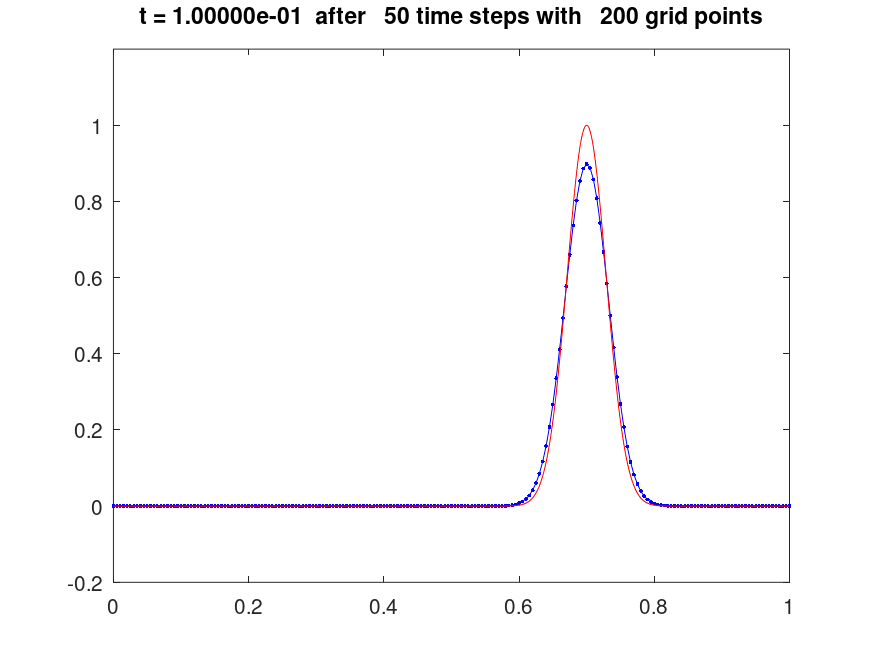
\includegraphics[width=\textwidth]{problem_3c_alpha-0.40.png}
            \caption{$\alpha = 0.40$}
        \end{subfigure}
        \hfill
        \begin{subfigure}[b]{0.45\textwidth}
            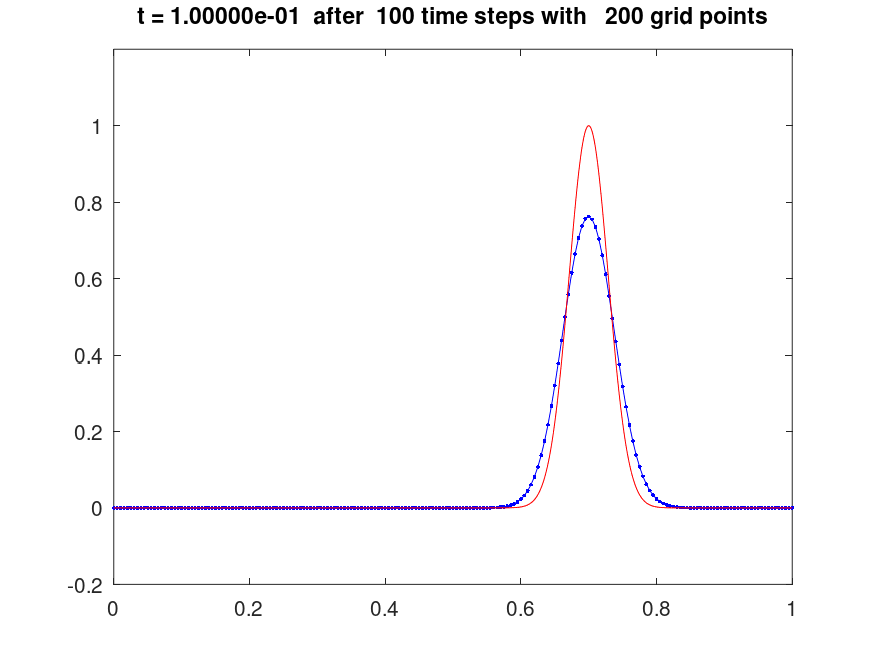
\includegraphics[width=\textwidth]{problem_3c_alpha-0.20.png}
            \caption{$\alpha = 0.20$}
        \end{subfigure}
        \hfill
        \begin{subfigure}[b]{0.45\textwidth}
            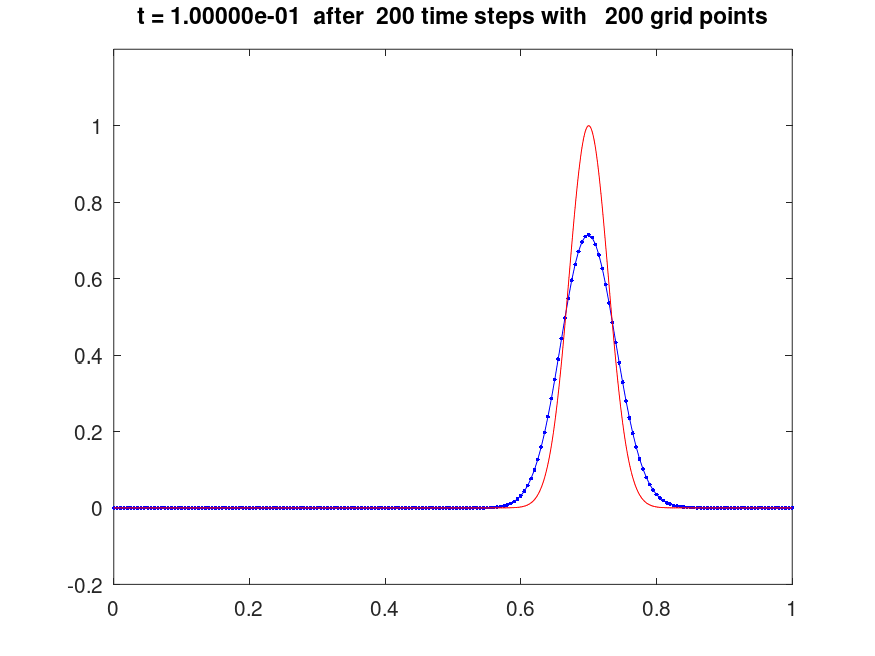
\includegraphics[width=\textwidth]{problem_3c_alpha-0.10.png}
            \caption{$\alpha = 0.10$}
        \end{subfigure}
    \end{figure}

    \pagebreak
    The second-order modified equation for the upwind method is given by LeVeque (10.44):
    
    $$
    v_t + av_x = \frac{1}{2}ah \left(1 - \frac{ak}{h}\right)v_{xx}
    $$

    As we decrease $k$ while holding $h$ fixed (that is, we examine the limit of the above PDE as $k \to 0$), our 
    modified PDE becomes:

    $$
    v_t + av_x = \frac{1}{2}ah v_{xx}
    $$

    which contains the diffusive term $\frac{1}{2} ah$ and accounts for the dampening error observed in the numerical 
    solution above.
    \ \\
\end{solution}